\begin{slide}{Swarm Algorithm Development}
  \begin{itemize}
  \item No methods for direct analysis of swarm algorithms
  \item Swarm algorithms evaluated through simulation
  \end{itemize}
  
  \vspace{2ex}

  Thus, a flexible swarm simulation platform is required.
  \begin{itemize}
  \item Multiple agent and swarm types
  \item Support for various environment types
  \item Access to all simulation data
  \item Easy to use
  \item Portable
  \end{itemize}
\end{slide}

%%%%%
%%%%%

\begin{slide}{\SWEEP}
  \SWEEP - \textbf{SW}arm \textbf{E}xperimentation and
  \textbf{E}valuation \textbf{P}latform
  
  \begin{minipage}{\textwidth}
    \centering
    \vspace{.5cm}
    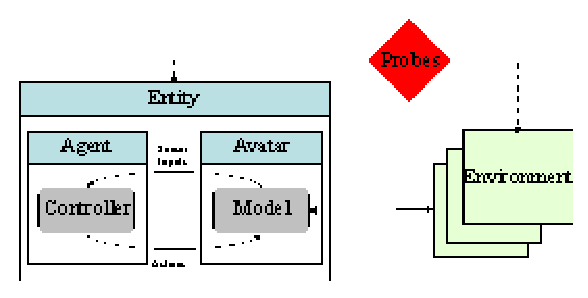
\includegraphics[scale=.35]{SweepDiagram.eps}
  \end{minipage}
\end{slide}

%%%%%
%%%%%

\begin{slide}{\SWEEP~- \texttt{Simulation}}
  \begin{minipage}{.65\textwidth}
    \begin{itemize}
    \item XML simulation specification file
    \item Responsible for constructing the simulation
    \item Handles update scheduling
      \begin{enumerate}
      \item \texttt{Environment}
      \item \texttt{Entity::Agent}
      \item \texttt{Entity::Avatar}
      \item \texttt{Probes}
      \end{enumerate}
    \end{itemize}
  \end{minipage}
  \hfill
  \begin{minipage}{.25\textwidth}
    \ttfamily
    \scriptsize
    \begin{tabbing}
      \hspace{1ex} \= \hspace{1ex} \= \kill
      $<$simulation$>$ \\
      \> $<$main/$>$ \\
      \> $<$agent/$>$ \\
      \> $<$controller/$>$ \\
      \> $<$model/$>$ \\
      \> $<$environment/$>$ \\
      \> $<$probes/$>$ \\
      $<$/simulation$>$ \\
    \end{tabbing}
  \end{minipage}
\end{slide}

%%%%%
%%%%%

\begin{slide}{\SWEEP~- \texttt{Entity::Agent}}
  The ``mind'' of the \texttt{Entity}
  \begin{itemize}
  \item \texttt{State}: collection of variables that define the agent
  \item \texttt{Controller}: defines the governing logic of the agent
  \item The default \texttt{Controller} is a finite state machine
  \end{itemize}
  
  \centering
  \begin{minipage}{.45\linewidth}
    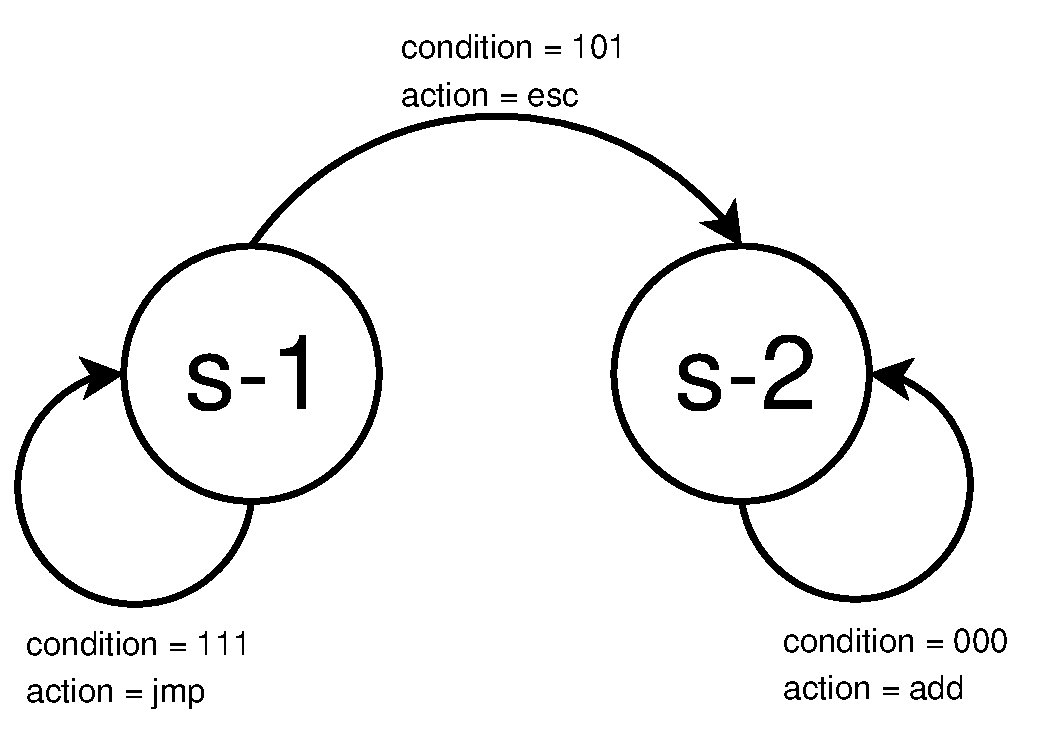
\includegraphics[scale=.3]{SimpleMachine}
  \end{minipage}
\end{slide}

%%%%%
%%%%%

\begin{slide}{\SWEEP~- \texttt{Entity::Avatar}}
  The ``body'' of the \texttt{Entity}
  \begin{itemize}
  \item Conduit between \texttt{Agents} and \texttt{Environments}
  \item Separates modeling and algorithm development
  \item e.g., a UAV
    \bigskip
  \item 
    \texttt{Model}: defines characteristics \\
    ~~~e.g., minimum turning radius, maximum thrust
  \item 
    \texttt{Sensor}: defines environmental information available\\
    ~~~e.g., chemical sensor, GPS
  \item 
    \texttt{Action}: defines behavioral abilities\\
    ~~~e.g., plan-path-to, return-to-base
  \end{itemize}
\end{slide}

%%%%%
%%%%%

\begin{slide}{\SWEEP~- \texttt{Environment}}
  The \texttt{Environment} has three core functionalities:
  \bigskip
  \begin{enumerate}
    \itemsep=3.5ex
  \item Defining fundamental laws that \texttt{Avatars} must respect\\
    ~~~e.g., gravity, $F=ma$, bandwidth limits
    
  \item Presenting an information abstraction layer\\
    ~~~e.g., neighborhood on a grid vs. a graph
    
  \item Facilitating direct and indirect communication\\
    ~~~e.g., simulating wireless, pheromone gradients
  \end{enumerate}
\end{slide}

%%%%%
%%%%%

\begin{slide}{\SWEEP~- \texttt{Probe}}
  \texttt{Probes} provide the ability to
  \begin{itemize}
  \item Extract information from a running simulation
  \item Inject information into a running simulation
  \end{itemize}
  
  \vspace{1em}
  
  The current \texttt{Probe} implementation uses \texttt{Connectors}.
  \begin{itemize}
  \item \texttt{Connectors} are data conduits between components
  \item \texttt{Probes} ``tap'' \texttt{Connectors}
  \item \texttt{Connectors} provide access to information injection/extraction
  \end{itemize}
  
  \vspace{1em}
  
  Example \texttt{Probe} usage: diagnostic interface
\end{slide}

%%%%%
%%%%%

\begin{slide}{\SWEEP Applications}
  This thesis:
  \begin{itemize}
  \item Dispersion
  \item Task assignment, CAST Auction
  \item \fbox{Chemical cloud tracking}
  \end{itemize}
  \bigskip
  Other works:
  \begin{itemize}
  \item Swarm reasoning for the four-color mapping problem
  \item Mars exploration using ``tumbleweeds''
  \item Extending swarm programming with aspect-oriented programming
  \end{itemize}
\end{slide}

